
\documentclass{informs3-noredtextontop}
\usepackage{enumerate}
\usepackage{interval}
\usepackage{float}
\intervalconfig{left open fence= (,right open fence=)}
\usepackage[ruled,vlined]{algorithm2e}
\usepackage{standalone}
\usepackage[style=base]{subcaption}
\usepackage{tikz}
\usetikzlibrary{arrows,shapes,positioning,decorations.pathreplacing,calc}
\usepackage{booktabs} % For \toprule, \midrule and \bottomrule
\usepackage{pgfplotstable} % Generates table from .csv
\usepackage[normalem]{ulem}
\newcommand{\stkout}[1]{\ifmmode\text{\sout{\ensuremath{#1}}}\else\sout{#1}\fi}
\usepackage{soul}
\usepackage{xcolor}
\pgfplotsset{compat=newest}


% Data of csv files
\pgfplotstableread[col sep=comma]{TUEserver_summary_opt.csv}\summaryopt{}

% \theoremstyle{TH}
\newtheorem{property}{Property}
\newtheorem{prop}{Proposition}
\makeatletter
\newcommand\footnoteref[1]{\protected@xdef{}\@thefnmark{\ref{#1}}\@footnotemark}
\makeatother

\OneAndAHalfSpacedXII% current default line spacing
%%\DoubleSpacedXII

% Natbib setup for author-year style
\usepackage{natbib}
%\bibpunct[, ]{}{}{,}{a}{}{,}%
 \def\bibfont{\small}%
 \def\bibsep{\smallskipamount}%
 \def\bibhang{24pt}%
 \def\newblock{\ }%
 \def\BIBand{and}%
%% Setup of theorem styles. Comment out only one.
%% Preferred default is the first option.
\TheoremsNumberedThrough% Preferred (Theorem 1, Lemma 1, Theorem 2)
%\TheoremsNumberedByChapter  % (Theorem 1.1, Lemma 1.1, Theorem 1.2)

%% Setup of the equation numbering system. Comment out only one.
%% Preferred default is the first option.
\EquationsNumberedThrough% Default: (1), (2), ...
%\EquationsNumberedBySection % (1.1), (1.2), ...

% In the reviewing and copy editing stage enter the manuscript number.
%\MANUSCRIPTNO{} % When the article is logged in and DOI assigned to it,
                 %   this manuscript number is no longer necessary

%%%%%%%%%%%%%%%%

\newcommand{\TWCT}{P||\sum_{j = 1}^n
w_jC_j}

\newcommand{\TWCTm}{P_m||\sum_{j = 1}^n
w_jC_j}

\theoremstyle{TH}

% Initialize data
\renewcommand{\theARTICLETOP}{}
\renewcommand{\RRHSecondLine}{}
\renewcommand{\LRHSecondLine}{}
\renewcommand{\theARTICLETOPRIGHT}{}
\renewcommand{\setoddRH}{\hbox to \textwidth{\fs.7.8.\tabcolsep0pt
  \begin{tabular*}{\textwidth}[b]{l@{\extracolsep\fill}r}
  {\theRRHFirstLine}&  \raisebox{0pt}[0pt][0pt]{\fs.10.10.\thepage}\\[-4pt]
  \rlap{\VRHDW{0.5pt}{0pt}{\textwidth}}&\\
  \end{tabular*}}}
\renewcommand{\setevenRH}{
	\hbox to \textwidth{\fs.7.8.\tabcolsep0pt
	  \begin{tabular*}{\textwidth}[b]{l@{\extracolsep\fill}r}
	   \raisebox{0pt}[0pt][0pt]{\fs.10.10.\thepage}&{\theLRHFirstLine}\\[-4pt]
	  \rlap{\VRHDW{0.5pt}{0pt}{\textwidth}}&\\
	  \end{tabular*}}
}

%%%%%%%%%%%%%%%%%%%%%%%%%%%%
%% command definitions    %%
%%%%%%%%%%%%%%%%%%%%%%%%%%%%
\newcommand*{\red}{\textcolor{red}}
\newcommand*{\green}{\textcolor{green}}
\newcommand*{\blue}{\textcolor{blue}}

\begin{document}

\section*{Performance profile curves}
\begin{figure}[t]
	\caption{Performance profiles over all the instances solved to optimality by both algorithms ($s = $ BDDF, ATIF)}\label{fig:overallpc}
	\centering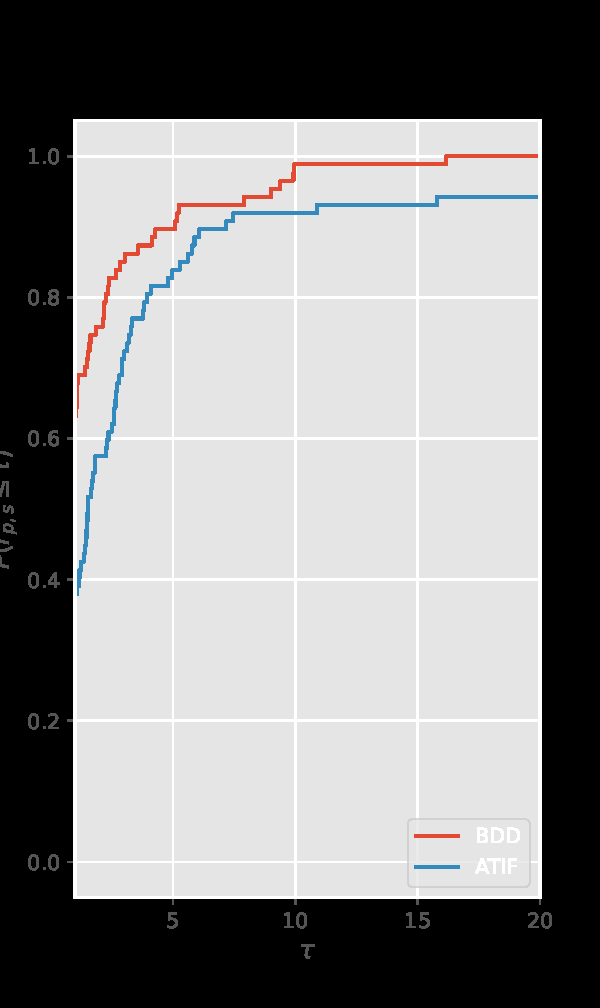
\includegraphics{profile_curve_overall.tex}
\end{figure}

\begin{figure}[t]
	\centering
	% \captionsetup[subfigure]{position=b}
	\caption{Performance profiles per instance class ($s = $ BDDF, ATIF)}\label{fig:per_instance_pc}
	\foreach \i/\j in {2/40, 4/40, 2/50, 4/50,2/100,4/100}{
			\subcaptionbox{\footnotesize{} \(\displaystyle m = \i \) and \(\displaystyle n = \j \)}{\resizebox*{0.45\textwidth}{!}{\includegraphics{profile_curve_\j_\i.tex}}}
		}
\end{figure}

\section*{Table}
\begin{table}[t]
	% \setlength{\tabcolsep}{4pt}
	\TABLE{Summary of the results for the exact procedures\label{tbl:summarybb}}{
		\pgfplotstabletypeset[
			columns={n,m,opt_TimeOliveira_mean_opt_func,OptFound_sum,opt_found_tot_bb_mean_opt_func,opt_sum,opt_tot_bb_mean_opt_func},
			every head row/.style={
					before row={%
							\toprule
							\multicolumn{2}{c}{}&  \multicolumn{2}{c}{ATIF}& \multicolumn{3}{c}{BDDF}\\
							\cmidrule(lr){3-4}\cmidrule(lr){5-7}
						},
					after row={\midrule},
				},
			% font=\scriptsize,
         every last row/.style={after row=\bottomrule},
			columns/n/.style={column type=r,int detect,column name=\textit{n}},
			columns/m/.style={column type=r,int detect,column name=\textit{m}},
			columns/opt_TimeOliveira_mean_opt_func/.style={column type=r,precision=2,zerofill,column name=\emph{avg time}},
			columns/OptFound_sum/.style={column type=r,column name=\emph{solved}},
			columns/opt_found_tot_bb_mean_opt_func/.style={column type=r,precision=2,zerofill,fixed,column name=\emph{avg time}},
			columns/opt_sum/.style={column type=r,fixed,column name=\emph{solved}},
			columns/opt_tot_bb_mean_opt_func/.style={column type=r,precision=2,zerofill,fixed,column name=\emph{avg time all}},
		]\summaryopt{}

	}{}
\end{table}
\end{document}